% !Mode:: "TeX::UTF-8"
\documentclass[slovensky]{svk}
\usepackage[round]{natbib}
\usepackage{subfig}
\usepackage{array}

\def\todo#1{\par\smallskip{\scriptsize {\bf TODO: }#1}\par\smallskip}

\def\ins{\mathop{\mathit{insert}}}
\def\find{\mathop{\mathit{find}}}
\def\delete{\mathop{\mathit{delete}}}
\def\dec{\mathop{\mathit{decreaseKey}}}
\def\delmin{\mathop{\mathit{deleteMin}}}
\def\meld{\mathop{\mathit{meld}}}
\def\rank{\mathop{\mathit{rank}}}
\def\L{\mathop{\mathit{left}}}
\def\R{\mathop{\mathit{right}}}
\def\reverse{\mathop{\mathit{reverse}}}
\def\Bp{$\hbox{\rm B}\!^+\!$}

\begin{document}
  \catcode`\"=\active \def "{\begingroup\clqq\def "{\endgroup\crqq}}

\title{Gnarley Trees: vizualizácia dátových štruktúr}

\author{
  Katka Kotrlová % \email{katka.kotrlova@gmail.com}
  \and 
  Pavol Lukča % \email{palyho mail}
  \and
  Viktor Tomkovič % \email{viktor.tomkovic@gmail.com}
  \and 
  Tatiana Tóthová % \email{táničkin mail}
}

\supervisor{
  Jakub Kováč %\email{kuko@ksp.sk}
  \email{algvis@googlegroups.com}
}

%% nasleduje kratka verzia nazvu clanku a 
%% zoznam autorov (bez krstnych mien)
%% tieto informacie sa zobrazuju v hlavicke
\titlerunning{Gnarley Trees -- vizualizácia dátových štruktúr}
\authorrunning{Kotrlová, Lukča, Tomkovič, Tóthová}

\institute{
Katedra informatiky,
FMFI UK,
Mlynská Dolina,
842~48~Bratislava}

\maketitle

\begin{abstract}
V článku prezentujeme našu prácu na projekte Gnarley Trees, ktorý začal
Jakub Kováč ako svoju bakalársku prácu. Zaoberá sa dátovými štruktúrami
a ich vizualizáciou. Z vyvažovaných stromov to sú \Bp-strom, strom s prstom
a strom s reverzom, z háld $d$-árna a ľavicová halda, skew halda a párovacia
halda. Z iných štruktúr bol pridaný union-find problém a písmenkový strom (trie).
Okrem vizualizácie sme softvér doplnili o históriu krokov a operácií,
jednoduchšie ovládanie a tesnejšie vykresľovanie stromov.

\noindent
\textbf{Dostupnosť:} Softvér je voľne dostupný na stránke
           {\small\url{http://people.ksp.sk/~kuko/gnarley-trees}}.
\keywords{Gnarley Trees, vizualizácia, algoritmy a dátové štruktúry}
\end{abstract}

\section{Úvod}
Dátové štruktúry a algoritmy tvoria základnú, prvotnú časť výučby 
informatiky. Vizualizácia algoritmov a dátových štruktúr je grafické 
znázornenie, ktoré abstrahuje od implementačných detajlov a reprezentácie
v pamäti. Je teda vhodnou pomôckou pri výučbe i samoštúdiu. 

Ukážka nášho softvéru \emph{Gnarley Trees} je na obrázku~\ref{img:historia}.
Tento projekt začal ako bakalárska práca Jakuba Kováča \citep{kuko};
v tomto článku popisujeme nové dátové štruktúry, ktoré sme vizualizovali
a nové funkcie a vylepšenia, ktoré sme doplnili.

% Ako ľudia so záujmom o dátové štruktúry sme sa rozhodli pomôcť vybudovať 
% dobrý softvér na vizualizáciu algoritmov a dátových štruktúr a obohatiť 
% kompiláciu Jakuba Kováča \citep{kuko} o ďalšie dátové štruktúry. 
Z vyvažovaných stromov vizualizujeme
\emph{B$^+$-strom}, \emph{strom s prstom} a \emph{strom s reverzami}, z háld to sú \emph{d-árna 
halda}, \emph{ľavicová halda}, \emph{skew halda} a \emph{párovacia halda}. 
Taktiež vizualizujeme aj \emph{union-find problém} a 
\emph{písmenkový strom (trie)}. 

Okrem vizualizácie softvér prerábame a neustále vylepšujeme.
Doplnili sme ho o históriu krokov a operácií, jednoduchšie ovládanie
a veľa ďalších funkcií. Softvér je celý v slovenčine aj angličtine a je 
implementovaný v jazyku \texttt{Java}. Dostupný je na stránke
\hbox{\url{http://people.ksp.sk/~kuko/gnarley-trees}} vo forme appletov
s jednotlivými dátovými štruktúrami, a tiež vo forme samostatného programu,
ktorý obsahuje všetky dátové štruktúry a je určený na používanie offline.

Našou snahou je vytvoriť kvalitný softvér nezávislý od operačného systému, 
ktorý bude vyhovovať ako pomôcka pri výučbe ako aj pri samoštúdiu a bude
voľne prístupný. 

%\bigskip
Predchádzajúci výskum v oblasti pedagogiky
zatiaľ nedokázal úplne preukázať pedagogickú efektívnosť
vizualizácií \citep{shaffer}, avšak viacero štúdií potvrdilo zvýšený záujem
a zapojenosť študentov \citep{naps02, hundhausen02}.

Rozmach vizualizácie algoritmov priniesla najmä {\tt Java} a jej fungovanie 
bez viazanosti na konkrétny operačný systém. Kvalita iných existujúcich vizualizácií sa líši 
a keďže ide o ľahko naprogramovateľné programy, je ich veľa a sú pomerne 
nekvalitné \citep{shaffer}. 
Zbieraním a analyzovaním kvality sa venuje skupina AlgoViz (\hbox{\url{http://algoviz.org/}}).

Zaujímavé je pozorovanie, že určovanie si vlastného tempa pri vizualizácií 
je veľká pomôcka. Naopak, ukazovanie pseudokódu alebo nemožnosť určenia si
vlastného tempa (napríklad animácia bez možnosti pozastavenia), takmer 
žiadne zlepšenie neprináša \citep{shaffer,saraiya}.

%\bigskip
Zvyšok článku je organizovaný nasledovne: V sekcií 2 popisujeme implementované
vylepšenia týkajúce sa vizualizácie, grafiky a ovládania, v sekciách 3 až 6
nové dátové štruktúry, ktoré sme implementovali a vizualizovali: vyvážené
stromy, haldy, union-find a písmenkové stromy.

\begin{figure*}
\centering
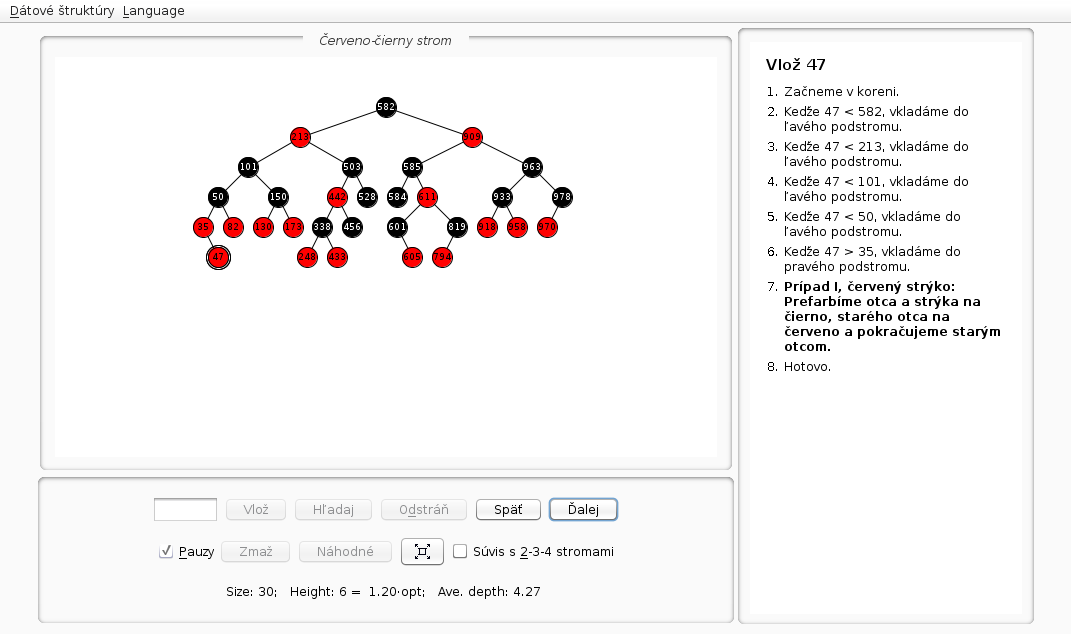
\includegraphics[width=2.01\columnwidth]{obrazky/gt.png}
\caption{\emph{Softvér Gnarley Trees.} V ovládacom paneli dole môže používateľ
zvoliť operáciu a vstupnú hodnotu a sledovať priebeh algoritmu (monentálne vkladanie
prvku 47). Používateľ postupuje vlastným tempom  pomocou tlačidiel \uv{Ďalej}, prípadne
\uv{Späť}. Vpravo je popis vykonávaných krokov; kliknutím na konkrétny krok v histórií
sa môže používateľ vrátiť.}
\label{img:historia} 
\end{figure*}

\section{Rozšírenie predošlej práce}

Projekt Gnarley Trees sme rozšírili nielen o vizualizácie ďalších dátových
štruktúr, ale pribudli aj softvérové (vizualizačné) vylepšenia:
kompaktnejšie vykresľovanie stromov, história krokov s možnosťou návratu,
či približovanie a vzďaľovanie.

\subsection{Tesnejšie vykresľovanie stromov}

V pôvodnej verzii programu sa stromy vykresľovali tak, že vertikálna súradnica 
predstavovala hĺbku v strome a horizontálna poradie vrcholu v~\emph{inorderovom
prechode} stromu (pozri obr.~\ref{img:rev1}). Tento jednoduchý spôsob však nešetrí priestor
a pri štruktúrach ako union-find či písmenkový strom by výsledné stromy 
vyzerali škaredo. Preto sme sa rozhodli pre stromy implementovať 
alternatívny spôsob rozloženia (pozri obr.~\ref{img:pairdel}), ktorý pre binárne stromy navrhli \citet{reingold}
a na všeobecné stromy rozšíril \citet{walker}. Tieto rozloženia vykresľujú
vrcholy stromov čo najtesnejšie, pričom dodržujú tieto estetické pravidlá: 
\begin{itemize} 
\item vrcholy v rovnakej hĺbke sú vykreslené na jednej priamke a priamky 
určujúce jednotlivé úrovne sú rovnobežné; 
\item poradie synov je zachované; 
\item otec leží v strede nad najľavejším a najpravejším synom; 
\item izomorfné podstromy sa vykreslia identicky až na presunutie;
\item ak vo všetkých vrcholoch obrátime poradie všetkých synov, výsledný strom 
sa vykreslí zrkadlovo.
\end{itemize}
Reingoldov-Tilfordov, aj zovšeobecnený Walkerov algoritmus pracuje v lineárnom
čase.

\subsection{História krokov}
Každá vizualizovaná operácia na dátovej štruktúre pozostáva
z niekoľkých krokov. Jednou z noviniek v projekte je možnosť vrátiť sa pri
prehliadaní operácií o niekoľko krokov späť, resp.\ vrátiť späť
celé operácie.

Niekedy sa stáva, že nedočkavý používateľ rýchlo prekliká cez celú vizualizáciu
a pritom si nestihne uvedomiť, aké zmeny sa vykonali na danej dátovej
štruktúre. Inokedy je operácia taká rozsiahla, že niektoré dôležité zmeny si
nevšimne. Vtedy by bolo užitočné pozrieť si vizualizáciu ešte raz (alebo
niekoľkokrát). Tento problém rieši história krokov. Používateľ má možnosť vrátiť
sa späť o jeden krok (tlačidlo "Späť"/"Previous") alebo preskočiť na ľubovoľný
krok po kliknutí na zodpovedajúci komentár (pozri obr.~\ref{img:historia}).

História krokov a operácií je atomická. Krok/operácia sa vykoná/vráti celý(-á)
alebo vôbec, pričom stav dátovej štruktúry korešponduje s pozíciou v histórii.
To umožňuje po vrátení celej operácie vykonať inú operáciu. Táto vlastnosť je
užitočná najmä v prípade vykonania operácie (prípadne zmazania celej dátovej
štruktúry) omylom.


\subsection{Ďalšie rozšírenia}
K ďalším rozšíreniam patrí možnosť priblíženia, vzdialenia a presunu vykreslenej dátovej štruktúry v rámci
vizualizačnej plochy. Používateľ túto funkcionalitu využije najmä pri dátových
štruktúrach s veľkým počtom prvkov, kedy je obmedzený veľkosťou plochy. Ďalším
rozšírením je výpis celej postupnosti komentárov vizualizovanej operácie,
ktorý prináša spolu s históriou krokov značné zjednodušenie
výučby. Používateľ si môže konkrétnu vizualizáciu pozrieť toľkokrát, koľko
potrebuje na jej správne pochopenie. Navyše vidí, aké kroky budú
nasledovať/predchádzať a podľa toho si môže určiť vlastné tempo prezerania
vizualizácie. Ak si myslí, že daným krokom už porozumel, môže ich preskočiť.


\section{Vyvážené stromy}

Pôvodná verzia \citep{kuko} obsahovala vizualizáciu viacerých vyvážených stromov.
K nim sme pridali \Bp-stromy, stromy s prstom a stromy s reverzami.

\subsection{B$\!^+\!$-strom}

\paragraph{Popis.}
\emph{\Bp-strom} je variácia B-stromu, v ktorom sú všetky kľúče uložené v listoch
a listy sú pospájané do spájaného zoznamu. Prvky vo vnútorných vrcholoch slúžia len
na navigáciu. 

\Bp-strom rádu $b$ je strom, v ktorom má každý vnútorný vrchol najviac $b$
a najmenej $\lfloor b/2 \rfloor$ synov (okrem koreňa, ktorý má najmenej dvoch synov).
Vďaka tomu je dobre vyvážený a jeho operácie sú vykonávané v logaritmickom čase.
\Bp-strom je \emph{asociatívne pole (slovník)}, čiže poskytuje tieto tri operácie:
\begin{itemize}
\item $\ins(x)$ -- pridá do stromu prvok $x$;
\item $\find(x)$ -- zistí, či sa $x$ v strome nachádza;
\item $\delete(x)$ -- odstráni $x$ zo stromu.
\end{itemize}

Operácia $\find(x)$ začne v koreni, nájde v ňom prvý kľúč väčší od hľadaného.
Nech je $i$-ty v poradí, potom hľadanie pokračuje $i$-tou vetvou.
(Ak je $x$ väčšie ako všetky kľúče, pokračujeme poslednou vetvou.)
V liste už len skontrolujeme, či sa v ňom hľadaný kľúč nachádza.

% Definujeme dve operácie: {\sc Copy-Up} a {\sc Push-Up}, ktoré používa operácia $\ins$.
% Ak má vrchol viac prvkov, ako je maximálny limit, treba ho zmenšiť. Rozdelí sa na dve časti.
% Ak vrchol nie je listom, použije sa {\sc Push-Up}, najmenší kľúč pravej časti sa vyberie
% a stane sa otcom vytvorených dvoch častí. Pokiaľ to list je, kľúč v ňom musí zostať,
% preto sa iba skopíruje. Táto operácia sa nazýva {\sc Copy-Up}.

Operácia $\ins(x)$ najprv pomocou operácie $\find$ zistí, či štruktúra daný kľúč už obsahuje.
Ak nie, je zrejmé, že $x$ patrí práve na miesto, kde $\find$ skončil.
Môže sa stať, že vrchol po vložení "pretečie" -- bude obsahovať $b+1$ prvkov. V takom prípade
ak má vrchol brata s menej ako $b$ prvkami, môžeme jeden kľúč presunúť k nemu.
Ak sú susedné vrcholy plné, vrchol rozdelíme na dva, pričom stredný kľúč skopírujeme
k otcovi. (Ten sa môže tiež preplniť -- môže vzniknúť celá kaskáda rozdelení, ktorá skončí
v najhoršom prípade v koreni.)
% Nový vrchol s jedným kľúčom, ktorý vznikol, vložíme do
% otcovského vrcholu. Ak otcovský vrchol presiahol najväčšiu možnú veľkosť, znova sa aplikuje
% popísaný algoritmus s jedným rozdielom -- namiesto {\sc Copy-Up} sa použije {\sc Push-Up}.

Podobne v operácií $\delete$ môže vrchol "podtiecť". Ak má suseda s aspoň $\lfloor b/2 \rfloor+1$
kľúčmi, môže si jeden požičať od neho. V opačnom prípade môžeme vrchol s jeho susedom zlúčiť.
% najprv pomocou $\find$ nájde kľúč, potom ho z vrcholu odstráni. Tento vrchol
% môže mať po odstránení menší počet kľúčov ako minimálny limit. Vtedy, ak sa dá, sa prenesie
% jeden kľúč zo súrodenca. Ak sa nedá, vrchol sa s ním zlúči. Zároveň sa k nim pridá aj kľúč
% z otcovského vrcholu, ktorý ich rozdeľoval. Pokiaľ to spôsobilo, že otcovský vrchol má menej
% kľúčov, ako je povolené, znova sa aplikuje predošlý algoritmus. Keďže na koreň sa nevzťahuje
% minimálny limit, po skončení bude strom zaručene v konzistentnom tvare.

\paragraph{Časová zložitosť a použitie.}
\Bp-stromy sú vhodnou dátovou štruktúrou pre dáta uložené na disku: keďže dĺžka prístupu na
disk je v porovnaní s výpočtami v hlavnej pamäti veľmi veľká, snažíme sa ich počet minimalizovať.
Hoci časová zložitosť všetkých operácií je $O(b\log_b n)$, potrebujeme iba $O(\log_b n)$ prístupov
na disk. Ak zvolíme vhodný rád, vieme jednotlivé vrcholy dobre napasovať na stránky a tým regulovať
ako počet prístupov k pamäti, tak jej zaplnenie.

Hlavné využitie \Bp-stromov je v databázových systémoch. Stromy vieme rozšíriť tak, aby podporovali
rôzne agregačné funkcie, ako napríklad súčet, minimum, či priemer daného intervalu pomocou $O(\log_b n)$
prístupov na disk. Vypísať všetky prvky z daného intervalu dokážeme pomocou $O(\log_b n + t/b)$ prístupov na disk.
% \Bp-strom podporuje efektívne vyhľadanie prvkov poľa, ktoré patria do daného intervalu.
% Algoritmus nájde jeden krajný bod a vďaka spájanému zoznamu, vytvorenému z listov, ostatné prvky
% postupne prečíta. Zložitosť je $O(\log_b(n) + t/b)$, kde $t$ je počet výsledných kľúčov z hľadaného intervalu.

Ďalšia výhoda \Bp-stromov oproti B-stromom sa prejaví, ak máme utriedený zoznam dát a chceme z neho vytvoriť \Bp-strom:
\Bp-strom môžeme vystavať odspodu. Takýto postup vyžaduje $O((n/b)\cdot\log_b n)$ prístupov na disk,
čo je $b$-krát rýchlejšie ako spraviť $n$ volaní $\ins$.

\begin{figure*}
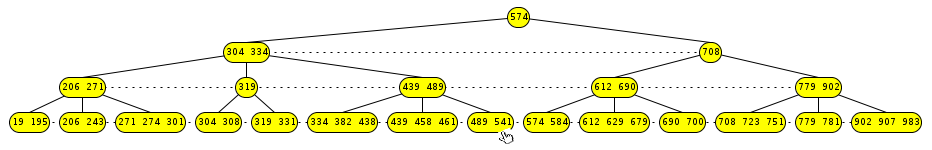
\includegraphics[width=2\columnwidth]{obrazky/finger.png}
\caption{\emph{Strom s prstom.} Jednotlivé kľúče sú uložené v listoch, vnútorné vrcholy
slúžia na vyhľadávanie. Vďaka smerníkom spájajúcim vrcholy na jednej úrovni vieme nájsť
ľubovoľný prvok vo vzdialenosti $d$ od prstu v čase $O(\log d)$.}
\label{img:finger}
\end{figure*}

\subsection{Strom s prstom}
Tradičné vyvážené vyhľadávacie stromy podporujú vyhľadávanie v čase $O(\log n)$.
Prst je smerník na konkrétny vrchol, ktorý umožňuje efektívnejší prístup k vrcholom
v jeho blízkom okolí. Hovoríme, že vyhľadávací strom podporuje vyhľadávanie s prstom
(tzv.\ \emph{finger search tree}), ak kľúč vo vzdialenosti $d$ dokážeme nájsť v čase $O(\log d)$.
Špeciálne predchodcu a následníka vieme nájsť v konštantnom čase.

Existuje viacero riešení, ktoré podporujú vyhľadávanie s prstom, v našom programe
sme implementovali upravený 2-3-4$^+$ strom \citep{finger}.

\paragraph{Popis.}
2-3-4$^+$ strom je \Bp-strom rádu 4, t.j.\ kľúče sú uložené v listoch a vnútorné vrcholy
majú stupeň 2, 3 alebo 4. Pre podporu vyhľadávania s prstom spojíme všetky vrcholy
na rovnakej úrovni (v rovnakej vzdialenosti od koreňa) do obojsmerného spájaného zoznamu.
Ak sú nejaké dva vrcholy spojené takouto hranou, budeme hovoriť, že sú susedia (pozri
obr.~\ref{img:finger}).

% Prst, ako už bolo spomenuté, ukazuje na nejaký vrchol. Môže sa pohybovať po všetkých hranách
% a pomocou neho sa vykonávajú všetky operácie. Keďže sú všetky kľúče uložené v listoch, prst
% na tejto vrstve začína, aj končí.

Operácia $\find$ začína vo vrchole, kam ukazuje prst. Vyhľadávanie pozostáva z dvoch
fáz: V prvej fáze postupujeme nahor, až kým hľadaný kľúč nepatrí do nášho alebo susedovho podstromu.
(V prípade potreby použijeme úrovňovú hranu, ktorou sa dostaneme do susedného vrcholu.)
V druhej fáze potom zostupujeme nadol ako pri štandardnom vyhľadávaní.
Pri $\ins$ a $\delete$ najskôr pomocou prstu nájdeme vhodné miesto a následne kľúč pridáme/vymažeme,
rovnako ako v \Bp-strome. 

Takto implementované vyhľadávanie trvá $O(\log d)$, vkladanie a vymazávanie (po tom ako sme vrchol
našli) má konštantnú amortizovanú zložitosť.


% Skontroluje, či by kľúč mal patriť do daného
% vrcholu. Ak nie, pozrie sa, či nepatrí do niektorého zo susedov. Ak áno, prst sa tam presunie
% a vyhľadávanie sa skončilo. Inak smerník prejde o úroveň vyššie, na otcovský vrchol. Ak hľadaný
% kľúč patrí do jeho podstromu (t.j.\ je väčší ako jeho najmenší kľúč a menší ako ten najväčší),
% zíde po hranách do listu, kde by sa daný kľúč mal nachádzať. Keď do podstromu nepatrí, skontroluje,
% či nepatrí do podstromu susedov. Ak áno, prejde po vrstevnej hrane na suseda a následne zíde až
% do listu, kde by mal kľúč byť. Pokiaľ prst nenarazil na správny podstrom, znova sa presunie smerom
% nahor po otcovskej hrane. Hľadanie pokračuje analogicky.
%Je zrejmé, že ak prst ukazuje na koreň, kľúč bude patriť do jeho podstromu.

% Otázka patričnosti do podstromu sa dá pre krajné prípady optimalizovať. Ak totiž vrchol, na ktorý
% ukazujeme, nemá napríklad pravého suseda, je zrejmé, že vačší kľúč ako je najvačší v tomto vrchole
% v strome nie je. Preto ľubovoľný kľúč do podstromu tohto vrcholu patrí práve vtedy, keď je väčší
% ako jeho najmenší prvok. Analogicky to platí, ak chýba ľavý sused.
% 
% Operácia $\ins$ najprv pomocou operácie $\find$ nájde miesto, kam by mal vkladaný kľúč patriť. 
% Ak taký kľúč už v strome je, ďalší sa nevloží. V prípade, že sme vložili nový kľúč, môže sa stať, 
% že vrchol "pretečie", tzn.\ má viac ako 3 prvky%
% (pozri obr.~\ref{img:finger-insert}). Situácia sa vyrieši rovnako ako v \Bp-strome. 

% Operácia $\ins$ najprv pomocou operácie $\find$ zistí, či štruktúra daný kľúč obsahuje. Ak nie, 
% je zrejmé, že patrí práve do vrcholu, kde $\find$ skončil. V prípade, že sme vložili nový kľúč, 
% môže sa stať, že vrchol "pretečie", tzn.\ má viac ako 3 prvky %
% (pozri obr.~\ref{img:finger-insert}). Ak vrchol pretiekol, použije sa {\sc Copy-Up}
% a rozdelí sa na dve časti. Stredný jednoprvkový vrchol sa vloží do otca. Ak pretiekol, použijeme 
% rovnaký postup, akurát s {\sc Push-Up}. Pokračujeme analogicky, pokým štruktúra nebude znova 
% v konzistentom stave.

% \begin{figure}
% 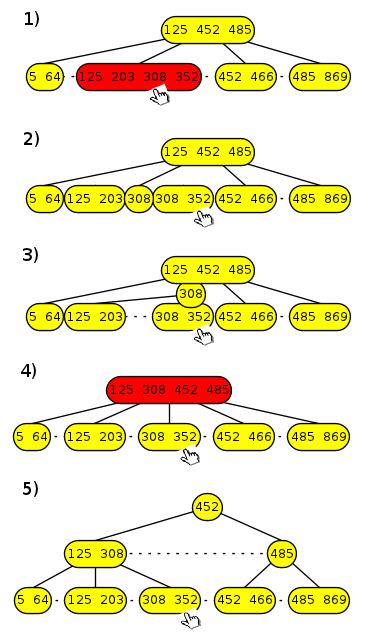
\includegraphics[width=\columnwidth]{obrazky/finger-insert.png}
% \caption{\emph{Pretečenie vrcholu.} Do stromu sme vložili prvok $308$ a 1) listový vrchol pretiekol. 
% 2) vrchol sa delí a kľúč sa kopíruje, aby originál zostal v liste 3) nový otec sa vkladá do vyššej vrstvy 
% 4) aj tento vrchol preteká, delí sa a vzniká nový koreň 5) finálny tvar.}
% \label{img:finger-insert}
% \end{figure}
% 
% Operácia $\delete$ najprv pomocou operácie $\find$ nájde miesto, kam by mal hľadaný kľúč patriť. 
% Ak tam nie je, vymazávanie sa končí. Inak sa vymaže. Môže sa stať, že vrchol "podtečie", tzn.\ 
% nemá kľúč. Tento problém sa rieši rovnako ako v \Bp-strome. 
% Samozrejme je treba ošetriť konzistentnosť vo vyšších vrstvách, aby sa tam nenachádzali kópie 
% kľúčov, ktoré už boli zo štruktúry vymazané (pozri obr.~\ref{img:finger-delete}).  
% 
% \begin{figure}
% 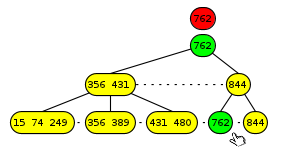
\includegraphics[width=\columnwidth]{obrazky/finger-delete.png}
% \caption{\emph{Vymazávanie kľúča $762$.} Odstrániť sa musí aj kópia vo vyšších vrstvách.}
% \label{img:finger-delete}
% \end{figure}
% 
% \paragraph{Časová zložitosť.}
% Keďže každý vrchol má aspoň dvoch synov, 2-3-4 strom má hĺbku $O(\log n)$, kde $n$ je počet kľúčov, 
% a teda podporuje vykonávanie operácií v čase $O(\log n)$. Ak sa však použije prst, časová zložitosť 
% vychádza na $O(\log d)$, kde $d$ je vzdialenosť pozície prsta a vrcholu, kam patrí cieľový kľúč, 
% amortizovane dokonca na $O(1)$ \citep{sahni}.

% \paragraph{Použitie.}
% Prst ako smerník na prvok štruktúry, ktorý umožňuje efektívnejší prístup k okolitým kľúčom, prvýkrát
% spomenuli Guibas et al. Vo svojej publikácii prezentujú B-strom podporujúci vyhľadávanie v $O(\log n)$
% a update-y dokonca v $O(1)$ čase, predpokladajúc, že je udržiavaných len $O(1)$ pohyblivých prstov \citet{sahni}.
% Pohyb prsta o $d$ pozícií trvalo $O(\log n)$ času. Na základe tejto práce navrhli Huddleston a Mehlhorn
% svoj vrstvovo spájaný 2-3-4 strom, ktorý bol neskôr upravený vďaka Belloch et al. na priestorovo efektívnejšiu
% alternatívu. Toto riešenie využíva jeden prst, s ktorým štruktúra ponúka rovnakú operačnú zložitosť ako 2-3-4 stromy.
% %Model bol dokonca zovšeobecnený na ($a$,$b$)-stromy, kde $b\geq 2a$.
% %Je zaujímavé, že pre 2-3 strom bola nájdená postupnosť vkladaní a vymazávaní, ktorá vyžaduje $\Omega(n\log n)$ krokov \citet{sahni}.

% \paragraph{Vizualizácia.}
% Strom s prstom je vizualizovaný pomocou \Bp-stromu s rádom 4, keďže jeho podmienky pre počet potomkov vyhovujú
% danej štruktúre.
% Prst je samostaný pohyblivý článok, ktorý si pamätá iba vrchol, na ktorý ukazuje. Po stromovitej
% štruktúre sa vie hýbať vďaka informáciám získaným z daného vrcholu.

\subsection{Strom s reverzami}
\emph{Strom s reverzami} je dátová štruktúra na uchovávanie permutácií. 
Majme permutáciu $\pi$ na množine $\{1,2,\ldots,n\}$; dátová štruktúra
poskytuje operácie 
\begin{itemize}
%\item $\ins(k)$ -- pridá do stromu $k$;
\item $\reverse(i,j)$ -- preklopí poradie prvkov v intervale od $i$ po $j$,
\item $\find(k)$ -- zistí, ktorý prvok je na $k$-tom mieste permutácie $\pi$.
\end{itemize}

\paragraph{Popis.}
Permutáciu reprezentujeme ako strom, v ktorom je \emph{inorder} poradie prvkov totožné 
s poradím prvkov v permutácií. Strom s reverzami môžeme implementovať pomocou ľubovoľného 
vyváženého stromu, ktorý podporuje rozdelenie a zreťazenie dvoch stromov v logaritmickom čase. 
My sme zvolili \emph{splay strom} pre jeho jednoduchosť. 

% Splay strom je štruktúrou binárny strom,
% líši sa od neho iba operáciami. Keď pracuje s ľubovoľným prvkom, na konci operácie bude vo vrchole
% buď daný kľúč alebo najbližší z jeho okoli. Na rozdiel od splay stromu, strom s reverzami nepracuje
% s kľúčmi, ale s poradím prvkov. Preto je nutné, aby mal

Niektoré vrcholy môžu byť označené vlajkou, ktorá signalizuje, že celý podstrom je reverznutý a 
prvky sú v skutočnosti v opačnom poradí (pozri obr.~\ref{img:rev1}).

Operáciu $\reverse$ implementujeme lenivo: 
strom najskôr rozdelíme na tri časti: $T_1,T_2,T_3$, pričom $T_2$ obsahuje interval od $i$-teho 
po $j$-ty prvok, $T_1$ obsahuje začiatok a $T_3$ koniec permutácie (obr.~\ref{img:rev2}). 
Koreň $T_2$ jednoducho označíme vlajkou. Ak už koreň vlajku obsahuje, odstránime ju. 
Následne stromy $T_1,T_2,T_3$ opäť spojíme.

Aby sme vedeli efektívne vyhľadať $k$-ty prvok, budeme si pre každý vrchol udržiavať veľkosť jeho
podstromu. V operácií $\mathop{\mathit{find}}(k)$ sa vieme podľa toho rozhodnúť, či sa $k$-ty prvok nachádza v ľavom podstrome,
resp.~koľký prvok je v pravom podstrome. (Po nájdení sa prvok presunie do koreňa pomocou operácie splay.)

\begin{figure}
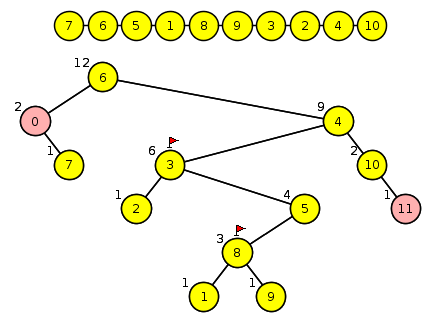
\includegraphics[width=\columnwidth]{obrazky/rev1.png}
\caption{\emph{Strom s reverzami.} Hore permutácia $\pi$, dolu jej reprezentácia pomocou splay stromu.
Vlajky vo vrcholoch 3 a 8 signalizujú, že v inorder poradí vrcholov $7,6,\underline{2,3,\underline{1,8,9},5},4,10$
treba podčiarknuté úseky (zodpovedajúce podstromom 3 a 8) prevrátiť.
Číslo vľavo hore od vrcholu je počet vrcholov v danom podstrome.}
\label{img:rev1}
\end{figure}

Pri takomto riešení musíme ešte upraviť vyhľadávanie a rotácie, aby brali do úvahy vlajky vo vrcholoch.
Najelegantnejšie riešenie je odstrániť vlajku vždy, keď na ňu narazíme:
Danému vrcholu odstránime vlajku, vymeníme mu synov a každému synovi vlajkový bit znegujeme.

Všetky operácie vieme implementovať v rovnakom čase ako operácie v splay tree, teda amortizovaná 
časová zložitosť oboch operácií je $O(\log n)$.

\paragraph{Použitie.}
Stromy s reverzami (pôvodne založené na AVL stromoch) navrhli \citet{chrobak}
na efektívnu implementáciu 2-opt heuristiky na riešenie problému obchodného cestujúceho.
Pri 2-opt heuristike sa snažíme preklápať rôzne úseky cesty, kým nenájdeme lokálne minimum.

V bioinformatike sa tieto stromy používajú na triedenie orientovaných permutácií
pomocou reverzov \citep{reversals,reversals2}.

Za povšimnutie stojí fakt, že táto dátová štruktúra podporuje výmenu ľubovoľných dvoch blokov
v logaritmickom čase, keďže túto operáciu vieme odsimulovať pomocou štyroch reverzov.

\paragraph{Vizualizácia.}
Pre lepšiu predstavu, bolo pridané pole, v ktorom používateľ vidí skutočné poradie prvkov, ktoré
zo stromu nie je až tak zjavné (obr.~\ref{img:rev1}, \ref{img:rev2}). Pole simuluje operácie spolu so stromom,
tie sa však vykonávajú v lineárnom čase.

Do stromu sme pridali ako zarážky prvky 0 a $n+1$. Tieto prvky do reverzovateľného
intervalu nepatria, majú však zmysel v prípade, ak sa reverzuje interval, ktorý zahŕňa
aspoň jeden okraj: V tom prípade v operácii $\reverse$ nezostane $T_1$ ani $T_3$ prázdny. 
%Aby nevznikli problémy s operáciami, za krajné kľúče boli zvolené hodnoty $0$ a číslo o jedna väčšie od aktuálneho maxima.

\begin{figure}
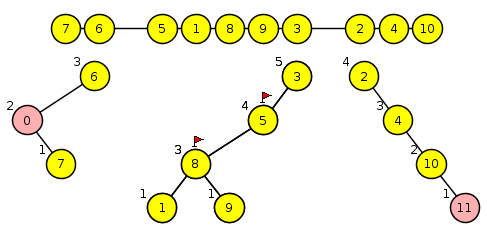
\includegraphics[width=\columnwidth]{obrazky/rev2.png}
\caption{Pri operácii \emph{reverse} sa strom rozdelí na tri časti. 
Vľavo sú prvky pred intervalom, vpravo prvky za ním. 
Na prevrátenie úseku $5,1,8,9,3$ stačí pridať vlajku vrcholu 3 (koreň stredného stromu)
a stromy opäť spojiť.}
\label{img:rev2}
\end{figure}


\section{Haldy}

V nasledujúcom texte sa budeme zaoberať rôznymi druhmi prioritných front. Popíšeme \emph{$d$-árnu haldu} ako 
základnú modifikáciu binárnej haldy, \emph{ľavicovú haldu} a niektoré druhy samoupravujúcich sa háld, konkrétne 
\emph{skew haldu} a \emph{párovaciu haldu}.
Halda je vo všeobecnosti \emph{zakorenený strom} s vrcholmi obsahujúcimi kľúče reprezentujúce dáta. Dôležitá je 
zakladná podmienka haldy, ak vrchol $p(x)$ je otcom vrcholu $x$, potom
$\hbox{\emph{kľúč}}(p(x)) \leq \hbox{\emph{kľúč}}(x)$\footnote{Bez ujmy na všeobecnosti budeme uvažovať o \emph{min haldách},
teda v koreni sa bude nachádzať najmenší prvok. Podobnými úvahami by sme text mohli rozšíriť o \emph{max haldy}
s najväčším prvkom v koreni.}.

Štandardné operácie, ktoré haldy podporujú, a ktorými sa budeme zaoberať pri každej dátovej štuktúre, sú:
\begin{itemize}
%\item $\mathop{\mathit{createHeap}}$ -- vytvorí prázdnu haldu;
\item $\ins(x)$ -- vloží vrchol s kľúčom $x$;
\item $\mathop{\mathit{findMin}}$ -- vráti minimum, t.j.~hodnotu kľúča v koreni;
\item $\delmin$ -- odstráni vrchol s najmenším kľúčom, t.j.~koreň;
\item $\dec(v, \Delta)$ -- zníži kľúč vrcholu $v$ o $\Delta\geq0$;
\end{itemize}

Niektoré haldy navyše implementujú operáciu $\meld(i, j)$, ktorá spojí haldu $i$ s haldou $j$.

\input haldy/daryheap.tex
\input haldy/leftist.tex
\input haldy/skewheap.tex
\input haldy/pairheap.tex

\def\null{\texttt{NULL}}
\def\makeset{$\mathop{\mathit{makeset}}(x)$}
\def\find{$\mathop{\mathit{find}}(x)$}
\def\union{$\mathop{\mathit{union}}(x, y)$}

\section{Union-find}

% Sú problémy, ktoré vyžadujú spájanie objektov do množín a množín navzájom 
% a následné určovanie, do ktorej množiny objekt patrí. Od takejto \emph{
% dátovej štruktúry pre disjunktné množiny} očakávame, že si bude udržiavať 
% jednoznačného \emph{zástupcu} každej množiny a bude poskytovať 
% tieto tri oprácie: 
V niektorých aplikáciach potrebujeme udržiavať prvky rozdelené do skupín
(disjunktných množín), pričom skupiny sa môžu zlučovať a my potrebujeme
pre daný prvok efektívne zistiť, do ktorej skupiny patrí. Predpokladáme,
že každá množina $S$ je jednoznačne určená jedným svojim zástupcom $x\in S$
a potrebujeme implementovať nasledovné tri operácie:

\begin{itemize}
\item \makeset\ -- vytvorí novú množinu $S=\{x\}$ s jedným prvkom; %,
                   %ktorý nepatrí do žiadnej inej množiny;
\item \union\ -- ak $x,y$ sú zástupcovia množín $S$ a $T$,
                 {\it union} vytvorí novú množinu $S\cup T$,
                 pričom $S$ aj $T$ zmaže. Zástupcom novej množiny $S\cup T$
                 je $x$ alebo $y$.
\item \find\ -- nájde zástupcu množiny, v ktorej sa 
                prvok $x$ nachádza.
\end{itemize}

%V takejto situácií je vhodná štruktúra \emph{union-find}.

% Vďaka častej asociácií objektov a spájania množín ako vrcholy a hrany grafu 
% sa často dátová štruktúra abstraktne reprezentuje ako 
% \emph{les} -- množina zakorenených stromov. 
% Konkrétnou implementáciou potom býva pole objektov -- vrcholov. Ku každému 
% objektu sa musí udržiavať smerník $p(x)$ na otca v strome. Smerník zástupcu 
% množiny ukazuje na hodnotu \null.

\paragraph{Použitie.}

Union-find sa dá použiť na reprezentáciu neorientovaného grafu,
do ktorého pridávame hrany a odpovedáme na otázku "sú dané dva
vrcholy spojené nejakou cestou?" (t.j.\ sú v rovnakom komponente súvislosti?).
Medzi najznámejšie aplikácie patria Kruskalov algoritmus na nájdenie najlacnejšej
kostry \citep{kruskal} a unifikácia \citep{unif}.

\citet{cholesky} ukázali, ako sa dá union-find použiť pri Choleského dekompozícií
riedkych matíc. Autori navrhli efektívny algoritmus, ktorý zistí počet nenulových
prvkov v každom riadku a stĺpci výslednej matice, čo slúži na efektívnu alokáciu
pamäte.

Pre offline verziu úlohy, kde sú všetky operácie dopredu známe, \citep{offline-uf}
navrhli lineárny algoritmus. Článok obsahuje tiež viacero aplikácií v teoretickej
informatike.

%\begin{figure}
%\includegraphics[width=\columnwidth]{obrazky/union.png}
%\caption{\emph{Spájanie podľa ranku.} (a) Pred spojením. (b) Po spojení. 
%Plytší strom sa napojil pod hlbší.} 
%\label{img:union} 
%\end{figure}

\paragraph{Popis.}
Dátová štruktúra \emph{union-find} sa reprezentuje ako les, kde každý strom zodpovedá
jednej množine a korene stromov sú zástupcovia množín. Pri implementácií si
stačí pre každý prvok $x$ udržiavať smerník $p(x)$ na jeho otca
(pre koreň je $p(x)=\null$).

Operácia \makeset\ teda vytvorí nový prvok $x$ a nastaví $p(x) = \null$. 

Operáciu \find\ vykonáme tak, že budeme sledovať cestu po smerníkoch, až 
kým nenájdeme zástupcu. 

Operáciu \union\ ide najjednoduchšie vykonať tak, že presmerujeme smerník 
$p(y)$ na prvok $x$, teda $p(y) \gets x$. 
Môžeme ľahko pozorovať, že takýto \emph{naivný} spôsob je neefektívny, 
lebo nám operácia \find\ v najhoršom prípade, na $n$ prvkoch, trvá $\Omega(n)$ 
krokov. 

\smallskip
Existujú dva prístupy ako zlepšiť operácie a tým aj zrýchliť ich vykonanie. 
Sú to: heuristika \emph{spájanie podľa ranku} a rôzne heuristiky na 
\emph{kompresiu cesty}. 

\paragraph{Heuristika na spájanie.}

Prvá heuristika pre každý vrchol $x$ udržuje hodnotu $\rank(x)$,
ktorá určuje najväčšiu možnú hĺbku podstromu s koreňom $x$.
Pri o\-pe\-rá\-cií \makeset\ zadefinujeme $\rank(x) = 1$. 
Pri o\-pe\-rá\-cií \union\ porovnáme $\rank(x)$ a $\rank(y)$
a vždy napojíme strom s menším rankom pod strom s väčším rankom.
Ak majú oba stromy rovnaký rank, napojíme povedzme $x$ pod $y$
a $\rank(y)$ zvýšime o 1.
%aby sme zistili, ktorý zástupca predstavuje menší strom. 
% Smerník tohto zástupcu potom napojíme 
% na zástupcu s výšším rankom. Zástupca novej množiny bude ten s vyšším rankom. 
% Ak sú oba ranky rovnaké, vyberieme ľubovoľného zo zástupcov $x$ a $y$, 
% jeho rank zvýšime o jeden a smerník ostatného zástupcu bude ukazovať 
% na tohto zástupcu. %Zástupcom novej množiny bude vybratý zástupca. 

\paragraph{Heuristiky na kompresiu cesty.}

\begin{figure}
\includegraphics[width=\columnwidth]{obrazky/komp.png}
\caption{\emph{Kompresia cesty z vrcholu 11 do koreňa.} 
Cesta je vyznačená šedou. 
(a) Pred vykonaním kompresie. Pri úplnej kompresii~(b) sa všetky vrcholy 
napoja na zástupcu. Pri delení cesty~(c) a pólení cesty~(d) sa cesta skráti 
približne na polovicu.} 
\label{img:komp} 
\end{figure}

Druhou heuristikou je kompresia cesty. Algoritmov na efektívnu kompresiu 
cesty je veľa \citep{paths2}, tu popíšeme tie najefektívnejšie. Prvou z nich 
je \emph{úplná kompresia} \citep{comp1}. Pri vykonávaní operácie \find, po tom, 
ako nájdeme zástupcu, napojíme všetky vrcholy po ceste priamo pod koreň (obr.~\ref{img:komp}(b)).
Toto síce trochu spomalí prvé hľadanie, ale výrazne zrýchli ďalšie hľadania pre
všetky prvky na ceste ku koreňu. Druhou heuristikou je \emph{delenie cesty} \citep{comp2}. Pri vykonávaní 
operácie \find\ pripojíme každý vrchol v ceste od vrcholu $x$ po koreň stromu
na otca jeho otca (obr.~\ref{img:komp}(c)). Treťou heuristikou je \emph{pólenie cesty} \citep{comp2}.
Pri vykonávaní operácie \find\  pripojíme každý druhý vrchol v ceste od vrcholu
$x$ po koreň stromu na otca jeho otca (obr.~\ref{img:komp}(d)).

Časová zložitosť union-findu záleží od toho, koľko prvkov je v množinách a koľko je 
operácií celkovo vykonaných operácií. Všetky uvedené spôsoby ako vykonať 
operáciu \find\ sa dajú použiť s obomi realizáciami operácie \union. 
Počet prvkov označme $n$ a počet operácií $m$. V praxi je zvyčajne počet 
operácií oveľa väčší ako počet prvkov. Pri tomto predpoklade ($m\geq n$) je 
pri použití spájania podľa ranku časová zložitosť pre algoritmus bez kompresie 
$\Theta(m\log n)$ a pre všetky tri uvedené typy kompresií 
$\Theta(m\mathop{\alpha}(m,n))$ \citep{paths2}.

\paragraph{Vizualizácia.}
Dátovú štruktúru union-find sme vizualizovali ako les. Pre názorné 
oddelenie množín sme si zvolili pravidlo, ktoré zakazovalo vykresliť vrchol 
napravo od najľavejšieho vrcholu a naľavo od napravejšieho vrcholu inej 
množiny. Jednotlivé množiny sme už vykreslovali tesným Walkerovým algoritmom 
\citep{walker}. Vizualizácia poskytuje všetky vyššie spomínané heuristiky a 
aj tlačidlo na vykonanie viacerých náhodných spojení naraz. Toto je užitočné, 
keď chce používateľ vidieť, ako dátová štruktúra vyzerá, po vykonaní 
veľa operácií.

% V tabuľke~\ref{fig:uf:comp} je porovnanie časových zložitostí \citep{paths2}.

% \begin{table}
% \centering
% \small
% %\footnotesize %toto tu mám nechať?
% \subfloat[Časová zložitosť pre union-find, keď $m \geq n$.][Prehľad časových zložitostí, ak $m \geq n$.]{
% \begin{tabular}{m{2.5cm}m{2.2cm}m{2.2cm}}
% & Naivné spájanie & Spájanie podľa ranku \tabularnewline
% \hline
% Naivné hľadanie & $\Theta\left( mn\right)$ & $\Theta\left( m\log n\right)$ \tabularnewline
% Úplná kompresia, delenie cesty, pólenie cesty & $\Theta\left(m\log _{1+m/n} n \right)$ & $\Theta\left( m\alpha\left( m, n\right) \right)$ \tabularnewline
% \label{fig:uf:comp1}
% \end{tabular}
% }
% \qquad
% \subfloat[Časová zložitosť pre union-find, keď $m < n$.][Prehľad časových zložitostí, ak $m < n$.]{
% \begin{tabular}{m{2.5cm}m{2.2cm}m{2.2cm}}
% & Naivné spájanie & Spájanie podľa ranku \tabularnewline
% \hline
% Naivné hľadanie & $\Theta\left( mn\right)$ & $\Theta\left(n + m\log n\right)$ \tabularnewline
% Úplná kompresia& $\Theta\left(n + m\log  n \right)$ & $\Theta\left(n + m\alpha\left( n, n\right) \right)$ \tabularnewline
% Delenie cesty & $\Theta\left(n \log m \right)$ & $\Theta\left(n + m\alpha\left( n, n\right) \right)$ \tabularnewline
% Pólenie cesty & $\Omega\left(n + m\log n \right)$, $O\left(n\log m\right)$ & $\Theta\left(n + m\alpha\left( n, n\right) \right)$ \tabularnewline
% \label{fig:uf:comp2}
% \end{tabular}}
% \caption{\normalsize Porovnanie časových zložitostí pre rôzne kombinácie hľadaní prvkov a 
% spájaní množín pre union-find. Počet prvkov je $n$ a počet operácií je $m$. $\alpha$ 
% je inverzná Ackermannova funkcia. V praxi zväčša platí, že $m > n$.}
% \label{fig:uf:comp}
% \end{table}

%citovat Walkerov alg. - to mám robiť tu?



\def\k{w}
%\def\kluc{kľúč}
\def\put{$\mathop{\mathit{insert}}(\k)$}
\def\find{$\mathop{\mathit{find}}(\k)$}
\def\delete{$\mathop{\mathit{delete}}(\k)$}
\def\trie{trie}
\def\uz{\hbox{\tt\$}}

\section{Písmenkový strom}
\emph{Písmenkový strom} reprezentuje množinu slov. Oproti binárnym 
vyhľadávacím stromom je hlavný rozdiel v tom, že kľúče nie sú uložené 
vo vrcholoch, ale samotná poloha v strome určuje kľúč (slovo). 

% My používame ako abecedu veľké znaky anglickej 
% abecedy a ukončovací znak značíme dolárom (\uz).



\paragraph{Popis.}
Písmenkový strom je \emph{zakorenený strom}, v~ktorom každá hrana obsahuje 
práve jeden znak z abecedy alebo \emph{ukončovací znak}. Teda, každá cesta 
z koreňa do listu so znakmi $w_1, w_2, \ldots, w_n, \uz$ prirodzene 
zodpovedá slovu $w=w_1w_2\cdots w_n$. \emph{Ukončovací znak} je ľubovoľný, 
dopredu dohodnutý symbol, ktorý sa v abecede nenachádza (napr. \uz). 

Písmenkový strom je \emph{asociatívne pole (slovník)}, čiže 
poskytuje tieto tri operácie:
\begin{itemize}
\item \put\ -- pridá do stromu slovo $\k$;
\item \find\ -- zistí, či sa v strome slovo $\k$ nachádza;
\item \delete\ -- odstráni zo stromu slovo $\k$.
\end{itemize}
Všetky operácie začínajú v koreni a ku slovu pridávajú ukončovací znak, 
teda pracujú s reťazcom $\k\uz$. 

Operácia \put\ vloží do stromu vstupný reťazec tak, že z reťazca číta znaky 
a prechádza po príslušných hranách. Ak hrana s daným symbolom neexistuje, 
pridá ju (pozri obr.~\ref{img:trieinsert}).

\begin{figure}
\includegraphics[width=\columnwidth]{obrazky/trieinsertsmall.png}
\caption{\emph{Vloženie slova \uv{{\tt SURNE}}.} Začiatok slova 
\uv{{\tt SU}} sa v strome nachádza, ešte treba pripojiť hrany 
so znakmi {\tt R}, {\tt N}, {\tt E} a \uz.} 
\label{img:trieinsert} 
\end{figure}

Operácia \find\ sa spustí z koreňa podľa postupnosti znakov. Ak hrana, 
po ktorej sa má spustiť neexistuje, dané slovo sa v strome nenachádza. 
Ak prečíta celý vstupný reťazec, dané slovo sa v strome nachádza.

Operácia \delete\ najprv pomocou operácie \find\ zistí umiestnenie slova. 
Ak sa slovo v strome nachádza, algoritmus odstráni hranu s ukončovacím 
znakom a vrchol, ktorý bol na nej zavesený. V tomto štádiu sa nám môže 
stať, že v strome ostane \emph{mŕtva vetva} -- nie je ukončená 
ukončovacím znakom. Pre fungovanie stromu to nevadí, všetky operácie by 
prebiehali správne, ale takto štruktúra zaberá zbytočne veľa miesta. 
Preto je dobré túto mŕtvu vetvu odstrániť (pozri obr.~\ref{img:triedelete}).

\begin{figure}
\includegraphics[width=\columnwidth]{obrazky/triedeletesmall.png}
\caption{\emph{Odstránenie slova \uv{{\tt PODLA}}.} Po odstránení 
\uz\ nám v strome ostane nepotrebá prípona \uv{{\tt DLA}} (mŕtva vetva), 
ktorá je vyznačená červenou.}
\label{img:triedelete} 
\end{figure}

\bigskip
% \paragraph{Časová zložitosť.}
Všetky tri operácie majú časovú 
zložitosť $O(|\k|)$, kde $|\k|$ je dĺžka slova.

\paragraph{Použitie.}
Prvýkrát navrhol písmenkový strom \citet{fredkin}, ktorý používal názov 
\emph{trie memory}\footnote{Z anglického re\emph{trie}val -- získanie.}, 
keďže išlo o spôsob udržiavania dát v pamäti. 
%používal operácie 
%$\mathop{storage}$ (\put), $\mathop{retrieval}$ (\find) 
%a $\mathop{deletion}$ (\delete) a dátovú štruktúru nazýval \emph{trie 
%memory}, keďže išlo naozaj o spôsob uloženia dát v pamäti.

%O niečo neskôr \citet{knuth} uviedol vo svojej knihe ako príklad na 
%písmenkový strom vreckový slovník. 
%V tom istom diele uviedol aj možnosť 
%komprimovania vetiev a možnosť prerobenia $m$-árneho \trie\ na binárny. 
%\citet{knuth} však ukázal len komprimovanie koncov vetiev. 
\citet{patricia} navrhol písmenkový strom, v ktorom sa každá cesta bez vetvení
skomprimuje do jedinej hrany (na hranách potom nie sú znaky, ale slová).
Táto štruktúra je známa pod menom \emph{PATRICIA} (tiež \emph{radix tree},
resp.\ \emph{radix trie}) a využíva sa napríklad v \emph{routovacích tabuľkách}
\citep{radix}.

Písmenkový strom (tzv.\ \emph{packed trie} alebo \emph{hash trie}) sa používa
napríklad v programe \TeX\ na slabikovanie slov \citep{liang}.
Pôvodný návrh \citep{fredkin} ako uložiť \trie\ do pamäte zaberal
príliš veľa nevyužitého priestoru. \citet{liang} však navrhol, ako
tieto nároky zmenšiť.

Písmenkové stromy sa podobajú na \emph{konečné automaty}. 
Vznikli rôzne modifikácie stromov na automaty, ktorých hlavnou výhodou je, 
že v komprimovanej podobe spájajú nielen predpony, ale aj prípony slov 
a teda v slovách ľudských jazykov výrazne znižujú pamäťový priestor potrebný 
na uchovanie dátovej štruktúry. Vďaka tomu sa využívajú na jazykovú korekciu, 
automatické dopĺňanie slov a podobne \citep{scrabble,ca}. 

Ďalšie použitie písmenkového stromu je pri triedení zoznamu slov. 
Všetky slová sa pridajú do stromu a potom sa spraví \emph{preorderový prechod} 
stromu. Túto myšlienku spracovali \citet{burstsort1} a veľmi výrazne zrýchlil 
triedenie dlhých zoznamov slov. Neskôr tento algoritmus vylepšili 
\citet{burstsort2}. Kvôli tomu, ako algoritmus pracuje, 
sa nazýva \emph{burstsort}.

% Špeciálnym použitím písmenkového stromu je vytvorenie stromu zo všetkých 
% prípon slova. Táto dátova štruktúra sa nazýva \emph{sufixový strom} a dá sa 
% mo\-di\-fi\-ko\-vať na udržiavanie viacerých slov. Tieto štruktúry majú 
% veľmi veľa praktických využití \citep{gusfield}. 

\paragraph{Vizualizácia.} Pri vizualizácií písmenkového stromu sme použili 
Walkerov algoritumus pre úsporné rozloženie vrcholov v strome
\citep{walker}. Keď má vrchol viacej synov a hrany kreslíme priamo, tak vzniká 
nedostatok priestoru pre umiestnenie znakov na hrany. Preto sme sa rozhodli 
kresliť hrany zakrivene, podľa Bézierovej krivky určenej štyrmi bodmi. 
Vo vizualizácií sa dajú vložiť náhodné slová podľa momentálne nastaveného 
jazyka. Taktiež sa automaticky odstraňuje diakritika a interpunkcia, takže 
sa dá naraz vložiť súvislý text.

\section{Záver}
%work in progress; co sme spravili - uz je v uvode?, preco sme lepsi - sme vobec lepsi (ako galles)?, 
%co este chceme/treba spravit - maybe DONE, co je rozrobene - v podstate to, co chceme spravit - same as previous?
%\\

V súčasnosti je málo programov, ktoré by prinášali komplexnejší prehľad 
využívaných dátových štruktúr. Na niektoré dokonca vizualizácia doposiaľ 
neexistuje. Je veľa appletov, ktoré implementujú niektoré algoritmy, avšak 
ich nedostatkom býva neprehľadnosť vizualizácie a hlavne okrem základných 
operácií dátovej štruktúry takmer žiadna interaktivita. 

Do budúcna sa plánujeme zaoberať vizualizáciou ďalších dátových 
štruktúr a program obohatíme aj o známe algoritmy. Plánujeme implementovať 
\emph{linking-cutting stromy}, \emph{intervalové stromy}, \emph{soft haldu} 
a niektoré \emph{perzistentné dátové štruktúry}.

Budeme pokračovať v dopĺňaní histórie krokov do všetkých dátových štruktúr, 
ale aj vo vylepšení používateľského rozhrania, refaktorovaní zdrojového kódu 
a inými softvérovými vylepšeniami. Našim cieľom je čo najviac zjednodušiť 
prácu s programom, spraviť ho čo najviac používateľsky prístupným a 
zrozumiteľným, a tak zefektívniť výučbu jednotlivých dátových štruktúr, 
resp.\ spraviť ju zábavnejšou.

\subsection{Príspevky autorov}
Katka Kotrlová obohatila projekt o vizualizácie $d$-árnej, ľavicovej, skew a 
párovacej haldy, Viktor Tomkovič pridal vizualizácie union-findu, písmenkového 
stromu a implementoval algoritmus na vykresľovanie všeobecných stromov, 
Tatiana Tóthová vizualizovala \Bp-strom, strom s prstom a strom s reverzami 
a Pavol Lukča dorobil históriu krokov a operácií do takmer všetkých slovníkov 
a venoval sa refaktorovaniu zdrojového kódu. Na príprave tohto textu sa 
podieľali všetci autori.


\input{podakovanie/podakovanie}

%\nocite{*}
\bibliographystyle{apalike}
\bibliography{references}

\end{document}
